\section{Results}\label{sec:results}

\subsection{Comparison with Large Models and Compact Detectors}\label{sec:comparison}

SpatialNet finds the wearer's hand reliably: its hand box reaches IoU${\geq}0.5$ in 92.6\% of test images, and its fingertip error is 3.9\,px at the $160\times160$ input (Appendix~\ref{app:heads}). The harder part is the target. Table~\ref{tab:main} places SpatialNet between two reference points.

\begin{table}[t]
  \caption{Target localisation on the EgoPoint test split (\%). Published results are copied, not re-run, and their protocols differ slightly from ours (Appendix~\ref{app:comparison}). The compact detectors were trained on the same split and scored by the same code as SpatialNet; the YOLO26n rows are our controlled runs (seed 42), and NanoDet-Plus-m comes from our benchmark. \emph{Centre in}: predicted target centre inside the labelled box. $^\dagger$\,Pretrained on COCO, the source of at least 41\% of the test images.}
  \label{tab:main}
  \footnotesize
  \setlength{\tabcolsep}{3.5pt}
  \begin{tabular}{lrrrrrr}
    \toprule
    Method & Params & GFLOPs & P@0.5 & P@0.7 & mIoU & Centre in \\
    \midrule
    \multicolumn{7}{l}{\emph{Large models trained on EgoPoint (published)}} \\
    \quad VistaRef, BEiT-3-L & $>$226M & -- & 93.9 & 82.6 & 82.0 & -- \\
    \quad PointVG-R, Qwen2.5-VL-7B, SFT + RL & 7B & -- & 83.6 & 74.5 & 75.7 & -- \\
    \quad Qwen2.5-VL-7B, SFT & 7B & -- & 63.6 & 56.7 & 59.8 & -- \\
    \multicolumn{7}{l}{\emph{Multimodal LLM without training on EgoPoint (published)}} \\
    \quad Qwen2.5-VL-7B, zero-shot & 7B & -- & 49.8 & 42.9 & 45.5 & -- \\
    \multicolumn{7}{l}{\emph{Compact detectors at the same compute (trained by us)}} \\
    \quad YOLO26n, 128\,px, ImageNet start & 2.50M & 0.225 & 62.9 & 43.4 & 56.4 & 82.1 \\
    \quad YOLO26n, 128\,px, COCO start$^\dagger$ & 2.50M & 0.225 & 64.4 & 45.5 & 58.3 & 82.2 \\
    \quad NanoDet-Plus-m, 160\,px, COCO start$^\dagger$ & 1.17M & 0.218 & 67.6 & 49.5 & 59.8 & 82.9 \\
    \midrule
    \textbf{SpatialNet}, 160\,px (deployed) & \textbf{0.72M} & 0.231 & 58.9 & 31.8 & 53.3 & \textbf{84.8} \\
    \quad same model, 320\,px input & 0.72M & 0.923 & 65.1 & 40.3 & 56.5 & -- \\
    \bottomrule
  \end{tabular}
\end{table}

\paragraph{Large models are far more accurate.} VistaRef places a correct box on the target in 94\% of test images, against 59\% for SpatialNet, and its boxes are much tighter. These models are 300 to 10{,}000 times larger and run on GPUs; SpatialNet gives up this accuracy for a model that runs on the glasses. Against a 7B multimodal LLM used without training on EgoPoint, SpatialNet finds the target more often (P@0.5 of 59 against 50\%) but draws looser boxes; given the protocol differences, we read this as the same accuracy range at a fraction of the size, not as superiority. The target head does real work: a box of mean size placed at the labelled fingertip reaches a P@0.5 of only 11\%, because target sizes vary widely (Appendix~\ref{app:comparison}).

\paragraph{At the same compute, compact detectors draw tighter boxes.} With the same ImageNet pretraining as our backbone, YOLO26n is 4.0 points higher in P@0.5 (95\% paired interval [2.2, 6.0]) and 11.6 points higher in P@0.7, and a second training seed gives the same picture. The COCO-pretrained detectors score higher still. The COCO overlap does not explain their lead: against the ImageNet start, the COCO start gains 2.4 points [0.6, 4.3] on the test images that do not come from COCO and nothing on those that do (Appendix~\ref{app:coco}), so its advantage is general transfer, not recall of the test photographs. Resolution narrows the gap, but only at a cost: SpatialNet at 320\,px reaches 65.1\% with four times the compute, where compact detectors improve too (COCO-pretrained YOLO26n at 192\,px reaches 69.9\% with 0.51 GFLOPs; Appendix~\ref{app:comparison}).

\subsection{Target Choice and Downstream Recognition}\label{sec:choice}

\paragraph{SpatialNet picks the labelled object more often.} Its predicted target centre lies inside the labelled box in 84.8\% of test images, against 81.6--82.2\% for the four controlled detectors, and every paired difference (2.6 to 3.2 points) has an interval that excludes zero. SpatialNet's deficit therefore lies in how far the object extends, not in which object it picks: in 26\% of the test images its box misses IoU 0.5 although its centre lies on the labelled object.

\paragraph{A recogniser names the object from its crops as often as from a detector's.} A ``what is that?'' assistant does not need a tight box; it needs the object's name. Table~\ref{tab:recog} shows how often each recogniser names the labelled category from a crop of each model's box. With both recognisers, SpatialNet's crops are named correctly as often as the detectors' crops: the paired differences lie between $-$1.3 and $+$0.3 points, and every interval includes zero and lies within $\pm$2.8 points. Localisation matters, since SpatialNet's crops are named correctly 6--8 points more often than the whole frame and reach about 90\% of the rate for crops of the labelled box. Its loose but well-centred boxes explain the result: they are still named correctly in 47--51\% of cases, close to the 54--58\% for boxes with IoU${\geq}0.5$. The exception is targets far from the fingertip, where the detectors' crops are named 4--8 points more often, in line with their better boxes there (Appendix~\ref{app:recog}).

\begin{table}[t]
  \caption{Downstream recognition: how often an off-the-shelf zero-shot recogniser names the labelled category from a crop of each model's target box, choosing among the 348 EgoPoint category names (top-1 accuracy, \%, on the 2,603 test targets with a category name). The labelled box and the whole frame are references. A box on a neighbouring object of the same category counts as correct.}
  \label{tab:recog}
  \footnotesize
  \begin{tabular}{lrr}
    \toprule
    Crop & CLIP ViT-B/16 & SigLIP base \\
    \midrule
    Labelled box (upper reference) & 53.9 & 59.4 \\
    Whole frame (lower reference) & 40.3 & 46.2 \\
    \midrule
    \textbf{SpatialNet} & 48.6 & 52.3 \\
    YOLO26n, ImageNet start (seeds 42 / 1) & 48.8 / 49.1 & 53.3 / 53.4 \\
    YOLO26n, ImageNet start + pasting & 49.9 & 52.0 \\
    YOLO26n, COCO start & 49.1 & 53.2 \\
    \bottomrule
  \end{tabular}
\end{table}

\paragraph{What this means.} For an application that needs a tight box, a compact detector is the better choice at this compute. For naming the target, SpatialNet does as well, and it also returns the hand, the fingertip and the direction from the same pass, with fewer parameters (0.72M, against 1.17M for NanoDet-Plus-m and 2.50M for YOLO26n). An interface can use these outputs for feedback, such as a fingertip cursor or the pointing ray, which helps mid-air pointing~\cite{mayer2018effect}, and for gating on hand presence. Whether users benefit from them, we did not test.

\subsection{What Matters at This Scale}\label{sec:design}

\paragraph{Input resolution is the largest lever.} Retraining the unchanged model at 224 and 320\,px raises P@0.5 from 58.9\% to 62.4\% and 65.1\%, a gain of 6.2 points at 320\,px (interval [4.4, 8.0]) at no parameter cost, against a spread of 0.1 points between seeds. A larger backbone does not help in the same way: MobileNetV3-Small and MobileNetV4-Conv-Small double or nearly triple the parameters without a significant change in P@0.5 (Appendix~\ref{app:backbone}). Extra compute is therefore best spent on the input. It costs two and four times the compute of the deployed model, which we have not yet measured on the glasses.

\paragraph{What each component adds.} Table~\ref{tab:ablation} retrains the 160\,px model without one component at a time. No component changes P@0.5 by more than 1.1 points; each adds a specific capability, at a cost of at most 13K parameters.
\begin{itemize}
\item \emph{Instance anchoring} (A4) makes the hand box and the direction more precise. Against a plain model of the same size, whose heads read a globally pooled feature, it improves the hand mIoU by 1.8 points [1.4, 2.2] and lowers the direction error by 3.4$^\circ$ [2.4, 4.5], both beyond the change from retraining.
\item \emph{Distractor pasting} (A1) keeps accuracy when other hands are in view. With one or two hands pasted into each test image, the model trained with pasting keeps 4.1 more points of P@0.5 [2.4, 5.8] and classifies 5.4 more points of no-hand frames correctly [1.9, 8.9], at no cost on clean images. The recipe is not specific to SpatialNet: YOLO26n trained with the same pasting becomes as stable as SpatialNet, whereas detectors trained without it lose 2.4--4.6 points of P@0.5 under pasted hands (Appendix~\ref{app:controlled}). Both tests use pasted hands, which resemble the training distribution; real bystander hands remain untested.
\item \emph{Explicit ray geometry} (A3) is not needed at this scale: removing the ray branch does not lower accuracy. Probing the trained model shows why. The branch has learned mainly that targets lie near the fingertip, which fits the 70\% of targets that the fingertip overlaps, rather than where the ray points, and neither restricting it to the space in front of the fingertip nor up-weighting targets away from the fingertip changes this (Appendix~\ref{app:ray}). We keep the branch in the deployed model because that is the model measured on the glasses.
\item The two \emph{consistency losses} (A2) sharpen the direction, not the box.
\end{itemize}

\begin{table}[t]
  \caption{Ablations at 160\,px (one training run each). First row: the full model; other rows: difference from it (points; degrees for the direction error, where positive means worse). \emph{Retraining}: the largest change that retraining the full model with seeds 1 and 2 produced. Bold: the 95\% paired interval excludes 0 and the difference exceeds the retraining row. $^\S$\,Not significant once duplicated test images are removed. \emph{With other hands}: one or two hands pasted into each test image. All columns are in Appendix~\ref{app:ablation}.}
  \label{tab:ablation}
  \footnotesize
  \setlength{\tabcolsep}{4pt}
  \begin{tabular}{lrrrrrr}
    \toprule
    & \multicolumn{4}{c}{Clean test images} & \multicolumn{2}{c}{With other hands} \\
    \cmidrule(lr){2-5}\cmidrule(l){6-7}
    Variant & P@0.5 & P@0.7 & Hand mIoU & Direction ($^\circ$) & P@0.5 & No hand kept \\
    \midrule
    Full model & 58.9 & 31.8 & 73.7 & 32.2 & 60.1 & 91.8 \\
    \quad Retraining (seeds 1, 2) & $\pm$0.1 & $\pm$0.8 & $\pm$0.3 & $\pm$1.2 & $\pm$0.4 & $\pm$3.3 \\
    \midrule
    A1 no distractor pasting & $-$0.1 & $-$1.3 & \textbf{$-$0.6} & \textbf{$+$1.8} & \textbf{$-$4.1} & \textbf{$-$5.4} \\
    A2 no consistency losses & $+$1.1 & $+$0.6 & $-$0.4 & \textbf{$+$1.5} & 0.0 & $-$1.2 \\
    A3 no ray branch & $+$0.7 & \textbf{$+$1.9}$^\S$ & 0.0 & \textbf{$-$1.3} & $+$1.0 & $+$1.2 \\
    A4 no instance anchoring & $-$0.3 & \textbf{$-$2.8}$^\S$ & \textbf{$-$1.8} & \textbf{$+$3.4} & $-$0.5 & 0.0 \\
    \bottomrule
  \end{tabular}
\end{table}

\subsection{On the Glasses}\label{sec:ondevice}

\begin{table}[t]
  \caption{Cost of the 160\,px model on the engineering unit of Section~\ref{sec:device}, with a server CPU for reference. The battery rows are single one-minute observations. $^\ast$\,Derived from the per-frame latency, assuming frames are processed back to back.}
  \label{tab:device}
  \footnotesize
  \begin{tabular}{lr}
    \toprule
    Measure & Value \\
    \midrule
    Glasses: inference latency per frame & 60--80\,ms \\
    Glasses: throughput$^\ast$ & 12--17 frames/s \\
    Glasses: peak additional RAM during inference & ${\approx}$100\,KB \\
    Glasses: battery drain in one minute, SpatialNet running continuously & 9\% \\
    Glasses: battery drain in one minute, streaming frames to the phone at 0.5\,fps & 16\% \\
    \midrule
    Server CPU (1 thread), PyTorch: latency, median & 25.7\,ms \\
    \bottomrule
  \end{tabular}
\end{table}

SpatialNet takes 60--80\,ms per frame on the glasses (Table~\ref{tab:device}), within the 100--200\,ms targeted for interactive response~\cite{miller1968response,card1991information}, and needs about 100\,KB of RAM beyond the idle application, with 1.6\,MB of FP16 weights. Running the weights in half precision gives the same target IoU as full precision on 320 validation images, so halving the model size costs no accuracy. Over one minute, continuous inference used 9 percentage points of charge, and streaming frames to the phone at 0.5\,fps used 16, although streaming sends one frame every two seconds while SpatialNet processes frames continuously. Each mode was measured once on an engineering unit without production power management, so this indicates the relative cost of the two modes on this unit only; it is not an energy measurement or a battery-life estimate. Continuous inference is the worst case: in use, the model would run only while the wearer points.

\subsection{Frames from the Glasses' Camera}\label{sec:realframes}

All accuracy figures above come from EgoPoint, whose images are mostly landscape and partly composed or edited. As a check of transfer to the deployed camera, \tbd{K} wearers recorded \tbd{N} frames with the glasses while pointing at everyday objects at different distances in \tbd{places}, and \tbd{M} frames with no hand in view. For each pointing frame, the wearer named the object they meant; afterwards, \tbd{two annotators} drew the boxes of that object and of the wearer's hand without seeing the model's outputs. We score the outputs that the model produced on the glasses with the metrics of Section~\ref{sec:metrics} and give Wilson intervals (Table~\ref{tab:real}); Figure~\ref{fig:real} shows examples. \tbd{One or two sentences on the result: whether the hand, the target and the centre in target stay close to the EgoPoint values, and which failure types of Section~\ref{sec:failures} appear.} With \tbd{N} frames, this check can reveal a large drop in accuracy but not a small one.

\begin{table}[t]
  \caption{The deployed model on EgoPoint and on frames from the glasses' camera, scored with the same metrics (\%; brackets: 95\% Wilson intervals). \emph{No hand kept}: frames without a hand classed as no hand, at the hand-gate threshold of 0.5.}
  \label{tab:real}
  \footnotesize
  \begin{tabular}{lrrrrr}
    \toprule
    Frames & Pointing / no hand & Hand P@0.5 & Target P@0.5 & Centre in & No hand kept \\
    \midrule
    EgoPoint test split & 2,604 / 425 & 92.6 & 58.9 & 84.8 & 93.4 \\
    Glasses' camera & \tbd{N} / \tbd{M} & \xx\ [\xx, \xx] & \xx\ [\xx, \xx] & \xx\ [\xx, \xx] & \xx\ [\xx, \xx] \\
    \bottomrule
  \end{tabular}
\end{table}

\begin{figure}[t]
  \centering
  \phfig{\linewidth}{3.2cm}{Six frames from the glasses' camera with SpatialNet's on-device outputs (hand, fingertip, ray, target) and the annotated target. Include at least one failure.}
  \caption{Frames from the glasses' camera. \tbd{Insert after the real-frame check.}}
  \Description{To be inserted: six photos from the glasses showing SpatialNet's outputs and the annotated target.}
  \label{fig:real}
\end{figure}

\subsection{Where SpatialNet Fails}\label{sec:failures}

We sorted the 558 test images with a target IoU below 0.3 by rule. In 36\% of them, the model found the right object but drew the wrong extent, for example part of a bed instead of the whole bed. In 33\%, the direction was wrong, and in 31\%, the model chose a neighbouring object despite a reasonable direction, typically a similar object next to the labelled one. The hand was missed in 1\%. Figure~\ref{fig:failures} shows four complex scenes: repeated tableware and a dense bookshelf create look-alike neighbours (a, b), foliage blurs the target's extent (c), and several depth layers separate the fingertip from the labelled boat (d). In all four, the wearer's hand and fingertip are found; the failure lies in deciding which object is meant and how far it extends. Some labels are themselves ambiguous, and such cases count as failures for every model alike. Single frames also produce false alarms: at threshold 0.5, the hand gate fires on 6.6\% of frames without a hand, although it separates the two kinds of frame with an AUROC of 0.998 (Appendix~\ref{app:heads}).

\begin{figure}[t]
  \centering
  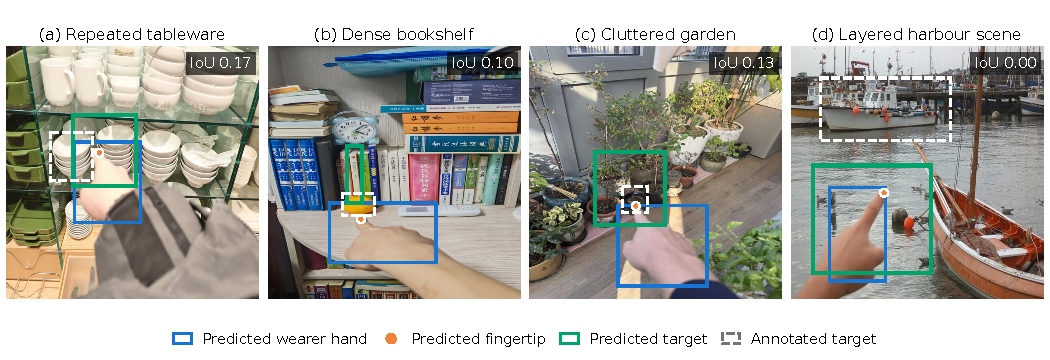
\includegraphics[width=\linewidth]{figures/failures_complex}
  \caption{Selected complex failures: repeated tableware (a) and a dense bookshelf (b) create look-alike neighbours; foliage complicates the target's extent (c); several depth layers separate the fingertip from the labelled boat (d). Colours as in Figure~\ref{fig:teaser}; boxes, points and IoUs are the saved test predictions of the 160\,px model.}
  \Description{Four egocentric photos where the predicted target box misses the labelled one: a box on the wrong stack of tableware in a glass cabinet (IoU 0.17), a box on a neighbouring book in a dense bookshelf (IoU 0.10), a box covering plants around a small object in a garden (IoU 0.13), and a foreground box instead of a distant boat in a harbour (IoU 0.00). The wearer's hand and fingertip are found in all four.}
  \label{fig:failures}
\end{figure}
